\documentclass[10pt]{article}
\title{Gegevensbanken - Samenvatting [H01O9A]\\*2010-2011}
\author{Wouter Schaekers\\*---\\*2Bach Informatica - 2Bach Fysica - 2Bach Biologie - 2Bach Ingenieurswetenschappen\\*3Bach Wiskunde - 3Bach Biochemie en Biotechnologie - 1-2Master Sterrenkunde}
\usepackage{amsmath}
\usepackage{graphicx}
\usepackage[top=25mm, bottom=25mm, left=25mm, right=25mm]{geometry}
\usepackage{color}
\usepackage{multicol}
\usepackage{listings}
\definecolor{gray}{RGB}{145,145,145}
\definecolor{brown}{RGB}{139,69,19}
\definecolor{blue}{RGB}{0,0,255}
\definecolor{green}{RGB}{0,100,0}
\definecolor{red}{RGB}{255,0,0}
\begin{document}
\maketitle
\setcounter{section}{-1}
\setcounter{page}{0}
\renewcommand{\contentsname}{Inhoudstafel}
\setcounter{tocdepth}{3}
\tableofcontents
\clearpage
\section{Inleiding en inhoudstafel}
Deze samenvatting is gemaakt voor de studenten van 2Bach Informatica, 2Bach Fysica, 2Bach Biologie, 2Bach Ingenieurswetenschappen, 3Bach Wiskunde, 3Bach Biochemie en Biotechnologie en 1-2Master Sterrenkunde.\\*
Deze samenvatting is gebaseerd op de slides die gebruikt zijn in de les. Daarom zal de aangehouden volgorde dezelfde zijn als de lessen, dus niet de volgorde van het boek. Redundante lessen worden weggelaten.\\*
In de samenvatting zal regelmatig verwezen worden naar afbeeldingen die in het boek staan. Hierbij is de zesde editie van het boek 'Database Systems' gebruikt.\\*
Deze samenvatting is hoogstwaarschijnlijk niet foutloos. Eventuele aanpassingen kunnen gemaakt worden op https://github.com/WouterSchaekers/Gegevensbanken-Samenvatting.\\*\\*
De auteur is niet bereid samenvattingen te signeren.\\*
Het sturen van spam is verboden. Het stalken van de auteur is, na toestemming, slechts in uitzonderlijke omstandigheden toegestaan.\\*
De auteur is niet verantwoordelijk voor enige gevolgen van het gebruik van deze bundel.\\*
Het is verboden de afgedrukte versie van de samenvatting te verbranden of op te eten.\\*\\*
Geen langdurig gebruik zonder wiskundig advies.\\*\\*
Alle lijnstukken voorbehouden.\\*
Niet op de openbare weg gooien.\\\\
This resume is released under the beerware license. Donations on the following bitcoin address are really appreciated. Thanks.\\\\\\\\\\\\\\\\\\\\\\\\\\\\\\\\
\begin{center}
\textit{"Alles moet zo eenvoudig mogelijk gemaakt worden, maar niet eenvoudiger dan dat."}\\*-\\*Albert Einstein
\end{center}
\begin{center}

\includegraphics[scale=0.5]{BitcoinAddress.png}\\*

\includegraphics[scale=0.02]{Bitcoin.png} \textbf{1Dh769mkyU3FGeEtxNcSQU4bSKkFZpFiPu}
\end{center}
\clearpage
\section{Het Relationeel Model}
\subsection{Inleiding}
\begin{center}
\begin{tabular}{ c c c c }
  Relatie & Attribuut 1 & Attribuut 2 & Attribuut 3\\
  Tupel 1 & Gegeven & Gegeven & Gegeven\\
  Tupel 2 & Gegeven & Gegeven & Gegeven\\
  Tupel 3 & Gegeven & Gegeven & Gegeven\\
\end{tabular}
\end{center}
Bijvoorbeeld, een anonieme vragenlijst ingevuld door informatici waarvan de gemiddelde resultaten bijgehouden worden:
\begin{center}
\begin{tabular}{ c c c c }
  Vakken & Moeilijkheid & Wekt interesse & Relevantie\\
  Logica & 6 & 9 & 8\\
  Wiskunde I & 1 & 6 & 7\\
  Wijsbegeerte & 5 & 1 & 0\\
  IOV & 7 & 5 & 3\\
  Gegevensbanken & 5 & 7 & 9\\
  Artifici\"ele intelligentie & 4 & 8 & 9\\
\end{tabular}
\end{center}
In dit geval zijn 'Moeilijkheid', 'Wekt interesse' en 'Relevantie' de attributen. 'Logica', 'Wiskunde I', \dots zijn de tupels.\\*
Op deze manier kunnen we uit deze tabel halen dat de gemiddelde informaticus het vak Wijsbegeerte niet interessant en absoluut niet relevant vindt.\\*
We noemen $U = \{A_1, A_2, \dots, A_n\}$ de verzameling van alle attributen en $DOM(A_i)$ de verzameling van alle mogelijke waarden voor $A$.\\\\
De formele notatie van een tupel kan op verschillende manieren gebeuren. We nemen in dit voorbeeld de eerste relatie van onze tabel:
\begin{center}
$<(Moeilijkheid, Wekt\ interesse, Relevantie), (6, 9, 8)>$\\*
$<(Moeilijkheid, 6), (Wekt\ interesse, 9), (Relevantie, 8)>$\\*
$(6, 9, 8)$\\*
\end{center}
Merk op dat alle waarden atomair zijn. Een waarde is atomair als deze niet meerwaardig of samengesteld is. $NULL$ waarden kunnen wel voorkomen.\\\\
Het is mogelijk dat je slechts een 'deeltupel' nodig hebt. In ons voorbeeld:
\begin{center}
$t =\ <6, 9, 8>$\\*
$t[Moeilijkheid, Relevantie] = (6, 8)$
\end{center}
\subsection{Het fysieke model}
Om een aantal begrippen te kunnen uitleggen gebruiken we het 'COMPANY' diagram (figuur 7.2 of zie slides).\\*\\*
Vierkante elementen zijn entiteiten en duiden meestal op een voorwerp of persoon. Ovale elementen zijn attributen, de eigenschappen van deze entiteiten. Ruitvormige elementen vormen de relaties tussen de entiteiten.
\subsection{Begrippen in verband met het model}
\textbf{Een regulier of sterk entiteitstype} Hangt niet af van een andere entiteit. Met andere woorden, een entiteit dat op zichzelf staat.\\*
\textbf{Een zwak entiteitstype} Hangt wel af van een andere entiteit. Deze entiteiten worden aangeduid met een dubbele rand.\\*
Bijvoorbeeld 'Employee' is een sterke entiteit, omdat dit een bepaalde persoon voorstelt (met een unieke id). Anderzijds is 'Team' een zwakke entiteit, omdat de identificatie van een team afhangt van het bedrijf waar het team onderdeel van is ('Team 1' kan in meerdere bedrijven voorkomen).\\
\textbf{Sleutelattribuut} Een attribuut dat een entiteit identificeert. Deze attributen worden onderlijnd.\\*
\textbf{Verwijssleutel} Een attribuut dan een zwakke entiteit identificeert. Deze attributen worden onderlijnd met een stippelijn.\\*
In het 'COMPANY'voorbeeld vinden we dat 'Ssn' het sleutelattribuut is van EMPLOYEE en 'Name' de verwijssleutel is van DEPENDENT.\\*
Sleutels moeten altijd uniek zijn.\\
\textbf{Binair relatietype} Een relatie tussen twee entiteiten. Deze kan $1:1$, $1:N$ en $N,M$ zijn en noemt ment de kardinaliteit. Deze wordt geschreven op de lijnen tussen de relaties. In dit voorbeeld kan een EMPLOYEE aan slechts \'e\'en DEPARTMENT werken en werken er aan \'e\'en DEPARTMENT meerdere EMPLOYEES. Vandaar de relatie $1:N$.\\
\textbf{Identificerende relatie} Relatie die een zwakke entiteit identificeert. Deze wordt aangeduid met een dubbele rand. In dit voorbeeld zal DEPENDENT worden ge\"identificeerd door EMPLOYEE.\\*
\textbf{Meervoudig attribuut} Een attribuut dat meerdere waarden kan hebben. Bijvoorbeeld DEPARTMENT kan meerdere locaties hebben. Meervoudige attributen hebben een dubbele rand. Dit mag niet verward worden met \textbf{Samengestelde attributen}. Deze attributen bestaan uit meerdere attributen die samen voorkomen. Bijvoorbeeld 'Geboortedatum' dat uit een dag, maand en jaar bestaat.\\*
\textbf{Afgeleide attributen} Deze attributen kunnen worden afgeleid uit andere attributen. Deze attributen zijn dus vrij redundant en kunnen eventueel weggelaten worden. Deze attributen worden omlijnd door een stippelijn. Bijvoorbeeld het attribuut 'omtrek' van een entiteit 'cirkel' terwijl het attribuut 'straal' al gegeven is.\\
\textbf{Totale participatie} Wanneer elk element van een bepaalde entiteit meedoet in een bepaalde relatie, is de participatie totaal. Dit wordt weergegeven door een dubbele relatie-lijn. In dit voorbeeld heeft elk DEPARTMENT een EMPLOYEE als manager, maar is niet elke EMPLOYEE een manager van een DEPARTMENT.\\
Een samenvatting van deze symbolen kan gevonden worden op figuur 7.14.

\subsection{Nog wat extra begrippen}
\textbf{Supersleutel} Een verzameling van attributen die een tupel ondubbelzinnig bepalen. Of anders gezegd: een set van attributen waarvoor geldt dat geen twee verschillende tupels dezelfde waarde hebben voor deze attributen.\\*
\textbf{Kandidaatsleutel} Een supersleutel zonder overtollige sleutel. Dus een zo klein mogelijke supersleutel.\\*
\textbf{Primaire sleutel} Een sleutel gekozen uit de kandidaatsleutel. De andere sleutels uit de kandidaatsleutel zijn \textbf{Alternatieve sleutels}. In ons model komt de primaire sleutel overeen met het sleutelattribuut. Deze primaire sleutel mag uiteraard nooit $NULL$ zijn.
\section{Het Entiteit Relatie Model (ER)}
Buiten binaire relatietypen kunnen er ook ternaire relatietypen opduiken. Dit is \'e\'en enkele relatie tussen drie entiteiten.
\begin{center}
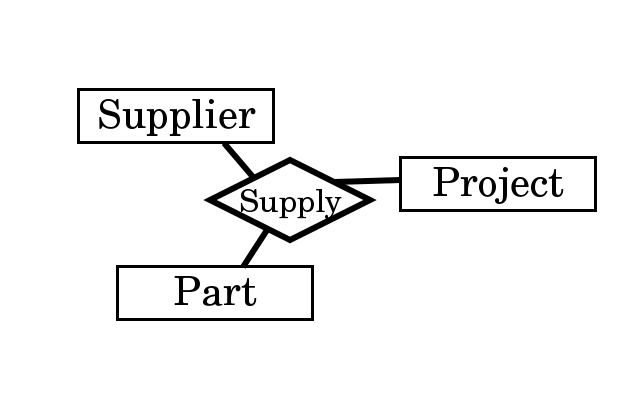
\includegraphics[width=85mm]{TernaireRelatie.png}\\*
\end{center}
\begin{center}
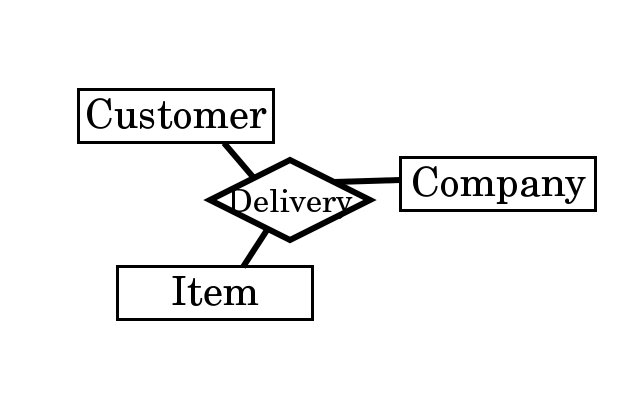
\includegraphics[width=85mm]{TernaireRelatie2.png}\\*
\end{center}
Ternaire relaties kunnen ook worden voorgesteld door drie binaire. Zie figuur 7.17 of slides.\\\\
Een zwakke entiteit wordt ge\"identificeerd via een ander entiteitstype. Het is logisch dat de deelname in deze identificerende relatie totaal moet zijn. In dit geval zijn zowel de foreign key (de sleutel via welke sterke entiteit deze entiteit wordt ge\"identificeerd) en de partial key (de sleutel van deze entiteit zelf die een zekere vorm van identificatie is) een onderdeel van de primary key. Partial keys worden met een stippelijn onderlijnd.
\section{Het Extended Entity Relationship Model (EER)}
EER is een uitebreide versie van ER. EER behandelt ook (sub/super)klassen, specialisatie/generalisatie en overerving van attributen.
\subsection{Specialisatie}
Specialisatie en generalisatie zijn in feite niets anders dan overerving. Bij specialisatie wordt een bepaald attribuut opgeslitst in verschillende entiteiten. Algemene attributen blijven bij de 'superentiteit'. Deze entiteit wordt dan opgesplitst in 'subentiteiten' zoals in figuur 7.19 (of slides).
\subsection{Generalisatie}
Bij generalisatie wordt de omgekeerde beweging gemaakt. Entiteiten worden bij elkaar gezet om tot een algemene 'superentiteit' te verkrijgen. De structuur blijft hetzelfde als bij specialisatie.
\subsection{Formele notaties}
Klasse = verzameling van entiteiten\\*
$Z=\{S_1, S_2, \dots, S_n\}$ is een specialisatie van $G \Leftrightarrow \forall i: G/S_i$ is een superklasse/subklasse relatie.\\*
$Z$ is totaal indien $\cup S_i = G$, anders parti\"eel.\\*
$Z$ is disjunct indien $\forall i, j, i \ne j: S_i \cap S_j = \emptyset$, anders overlappend.\\*
Een categorie T is een deelverzameling van de unie van haar superklassen: $T \subseteq D_1 \cup D_2 \cup \dots \cup D_n$
\section{Relationele algebra en relationele calculus}
Het opstellen van een database is niet genoeg. Je moet er uiteraard ook iets mee kunnen doen. Dat gaan we in dit en volgende hoofdstukken behandelen. Dit hoofdstuk heeft als doel een relationele taal (query language) op te zetten dat gebruikt kan worden om de database te manipuleren.\\*
De voorbeelden die gebruikt zullen worden, zullen gaan over figuur 3.6.
\subsection{Relationele algebra}
\subsubsection{Selectie}
Selectie van tupels (= rijen uit een tabel):\\*
$\sigma_{<Selectiecriterium>}(R)$\\*
In dit selectiecriterium mogen de volgende logische symbolen gebruikt worden: 
$=, \ne, <, >, <=, >=, \wedge, \vee, \neg$\\*
Merk op dat een opeenvolging van selecties ook voorgesteld kan worden door een conjunctie van deze beperkingen:\\*
$\sigma_3(\sigma_2(\sigma_1(R))) = \sigma_{1 \wedge 2 \wedge 3}(R)$\\\\
Voorbeeld:\\*
$\sigma_{Salary > 40000}(EMPLOYEE)$\\*
Dit levert de vierde en achtste rij van de relatie EMPLOYEE.\\*
\subsubsection{Projectie}
Selectie van kolommen.\\*
$\pi_{<Attributenlijst>}(R)$\\*
Dubbele tupels worden verwijdert, waardoor de kardinaliteit kan dalen (ze kan in ieder geval niet stijgen).\\*
Een opeenvolging van projecties $\pi_Y(\pi_X(R))$ is idempotent (enkel de laatste, buitenste projectie moet namelijk uitgevoerd worden, de binnenste projecties zijn dus redundant) en kan enkel indien:\\*
$Y \subseteq X$ (anders worden er attributen gebruikt die niet meer bestaan)\\\\
Voorbeeld:\\*
$\pi_{Fname, Lname}(EMPLOYEE)$\\*
Dit levert de eerste en derde kolom.
\subsubsection{Combinaties}
Uitdrukkingen kunnen gecombineerd worden:\\*
$\pi_{Fname, Lname}(\sigma_{Salary > 40000}(EMPLOYEE))$ (Geef de voor- en achternaam van de werknemers die meer dan 40000 verdienen.)\\*
Dit levert volgende tabel:\\*\begin{center}
\begin{tabular}{| c | c|}
\hline
Fname & Lname\\ \hline
Jennifer & Wallace\\ \hline
James & Borg\\ \hline
\end{tabular}
\end{center}
Er kan ook gebruik gemaakt worden van variabelen:\\*
$SELECTION = \sigma_{Salary > 40000}(EMPLOYEE)$\\*
$RESULT = \pi_{Fname, Lname}(SELECTION)$\\
Hernoeming is ook mogelijk:\\*
$SELECTION(Firstname, Lastname) = \sigma_{Salary > 40000}(EMPLOYEE)$\\*
Uiteraard moet er dan met deze nieuwe namen voortgewerkt worden.\\\\
Het gebruik van unie $\bigcup$ , doorsnede $\bigcap$ en verschil $\not\ \ $ is toegestaan indien mogelijk (Beide relaties moeten uiteraard dezelfde graad en domein hebben.). Dubbele tupels worden weggelaten.
\subsubsection{Carthesisch product}
$Q = R * S$\\*
Dit geeft alle mogelijk combinaties van tupels. (Indien $R$ 3 tupels heeft en $S$ 7, dan heeft $Q$ er 21.) Dubbele attributen blijven bestaan.
\subsubsection{Join operator}
$Q = R \bowtie_F S$\\*
Hetzelfde als het carthesisch product, enkel met een selectiecriterium.\\\\
Voorbeeld:\\*
DEPARTMENT $\bowtie_{DEPARTMENT.Dnumber = DEPT\_LOCATION.Dnumber}$ DEPT\_LOCATION\\*
Dit geeft vijf tupels.\\\\
Equi-join: Join waarbij enkel '=' wordt gebruikt in het criterium (zoals het bovenstaand voorbeeld).\\*
Natuurlijke join: Equi-join, waarbij overtollige attributen worden weggelaten. $Q = R *_F S$\\*
$F$ kan genoteerd worden als een conditie, maar ook als een attribuut, aangezien enkel gelijkheid mag worden gebruikt. Indien er geen attributen gegeven worden, wil dat zeggen dat alle overeenkomstige attributen gelijk moeten zijn.
\subsubsection{Deling}
$Q = R \div S$\\*
Het omgekeerde van het carthesisch product.\\*
$Q$ is de maximale relatie waarvoor geldt dat: $Q * S \subseteq R$\\*
$Q$ bevat enkel de attributen van $R$ die niet in $S$ zitten.
\subsubsection{Aggregaatfuncties}
Functies zoals $SUM, AVERAGE, MAX, MIN, COUNT$.\\*
$_{attributen}\Im_{functie}(R)$\\\\
Voorbeeld:\\*
$_{Dno}\Im_{MAX Salary}(EMPLOYEE)$\\*
Dit geeft de tabel van werknemers, gesorteerd op Dno, waarbij voor elke Dno het maximum salaris is weergegeven. (Er zijn dus drie tupels.)
\subsubsection{Uitwendige join}
De gewone join levert enkel informatie indien tupels aan een bepaalde voorwaarde voldoen. De uitwendige join wil deze tupels wel weergeven (dit geeft NULL waarden).\\*
Er zijn twee uitwendige joins: de linkse $Q = R\ ]\bowtie\ S$ en de rechtse $Q = R \bowtie[\ S$.\\\\
Voorbeeld:\\*
$EMPLOYEE\ ]\bowtie_{Ssn = Mgr\_ssn}\ DEPARTMENT$\\*
zal evenveel tupels leveren als EMPLOYEE er heeft (8), maar zal NULL waarden geven bij sommige attributen uit DEPARTMENT.\\*
De rechtse join zal 3 tupels leveren (en in dit geval geen NULL waarden bevatten).
\subsubsection{Varianten op unie}
$U^+$: De uitwendige unie (NULL waarden voor attributen die niet van toepassing zijn)\\*
$U^-$: Enkel gemeenschappelijke attributen blijven behouden.
\subsection{Relationele calculus}
Relationele calculus maakt gebruik van eerste orde predikatenlogica.\\*
Basisvorm van een query:\\*
$\{t.A_1, t.A_2, \dots, t.A_n|formule(t)\}$ ($A_i$ = attribuut)\\\\
Voorbeeld:\\*
$\{$t.Fname$|$EMPLOYEE(t) and t.Sex = 'M' and t.Salary $<$ 30000$\}$\\*
De betekenis van deze query is vrij triviaal en levert 'Ahmad' op.\\\\
In de relationele calculus kan gebruik worden gemaakt van quantoren ($\forall, \exists$), ontkenning ($\neg$), implicatie ($\Rightarrow$) en equivalentie ($\leftrightarrow$).
\section{SQL - Deel 1}
\subsection{Inleiding}
\subsubsection{Schema}
CREATE SCHEMA \textit{name}\\*
AUTHORIZATION \textit{name}
\subsubsection{Tabel}
CREATE TABLE \textit{name}\\*
(\textit{column name} \textit{column type} \textit{attribute constraint}\\*
\dots\\*
\textit{table constraint})\\*
\textit{column type}: Soort van variabelen (INT, FLOAT, DEC(i (precisie),j (schaal)), CHAR(n), VARCHAR(n), BIT(n), BIT VARYING(n), BOOLEAN, DATE, TIME, TIMESTAMP)\\
\textit{attribute constraint}:\\*
NOT NULL\\
\textit{table constraint}:\\*
PRIMARY KEY(\textit{attribute}),\\*
FOREIGN KEY(\textit{attribute}) REFERENCES \textit{TABLE(key)}
\subsubsection{Definitie van een attribuut}
CREATE DOMAIN \textit{attribute name} AS \textit{type}
\subsubsection{Restricties op tabel}
CONSTRAINT \textit{name}
PRIMARY KEY(\textit{attribute})
ON DELETE SET NULL ON UPDATE CASCADE (voer verandering door, om integriteit te bewaren)
\subsubsection{Drop behaviour (schema/tabel)}
CASCADE: Alles wordt weggelaten (inclusief eventuele views)\\*
RESTRICT: Enkel weglaten indien geen geen verwijzingen ernaar\\*
ALTER TABLE \textit{TABLE NAME}\\*
DROP COLUMN \textit{column name} CASCADE;
\subsection{Queries}
Algemene structuur:\\*
SELECT \textit{attributen} (projectie)\\*
FROM \textit{tabel(len)} (carthesisch product)\\*
WHERE \textit{condities} (selectie)
\subsubsection{Dubbele attribuutnamen}
In het geval van dubbele attribuutnamen: \textit{tabel}.\textit{attribuut}
\subsubsection{Aliasen}
SELECT E.Ssn, S.Ssn\\*
FROM EMPLOYEE AS E, EMPLOYEE AS S\\*
WHERE \dots
\subsubsection{DISTINCT}
SQL elimineert niet automatisch alle dubbele tupels.\\*
Vandaar het gebruik van DISTINCT.\\*
SELECT DISTINCT \textit{attribute}\\*
\dots
\subsubsection{Verzamelingen-bewerkingen}
UNION, INTERSECT, EXCEPT\\*
(SELECT \dots) \textit{BEWERKING} (SELECT \dots)\\*
Gebruik het sleutelwoord ALL na een bewerking indien gewerkt wordt met multisets (members zijn niet uniek).
\subsubsection{LIKE}
Patroonherkenning.\\*
\dots\\*
WHERE Date LIKE '2011\_\_\_\_'
\subsection{Operatoren}
+,-,*,/ kunnen ook gebruikt worden.\\*
Net zoals concatenatie (voor strings): $||$\\*
BETWEEN: BETWEEN 1 and 3\\*
ALL en ANY: a < ANY b (c 
\subsection{Gegevens ordenen}
\dots\\*
WHERE \dots\\*
ORDER BY \textit{attribute} [ASC/DESC]
\subsection{Geneste queries}
De IN operator: duidt aan dat een tupel in een bepaalde verzameling zit.\\*
SELECT \dots\\*
FROM \dots\\*
WHERE \dots IN (SELECT \dots)
\section{SQL - Deel 2}
Deel 2 gaat over geavanceerdere concepten dan in het vorige hoofdstuk werden behandeld.
\subsection{CONTAINS}
'Heeft als deelverzameling.' (niet meer ge\"implementeerd in de meeste versies van SQL)
\subsection{EXISTS}
EXISTS(\textit{verzameling}) geeft 1 terug als de verzameling niet leeg is, 0 in het andere geval.
\subsection{Expliciete verzamelingen}
\dots\\*
WHERE \textit{attribute} IN (1, 2, 3)
\subsection{Join operaties}
'FROM' is een join operatie. Deze operaties kunnen ook expliciet opgeschreven worden.\\*
FROM \dots NATURAL JOIN \dots
\subsection{Aggregaatfuncties}
COUNT, SUM, MAX, MIN, AVG\\*
SELECT \textit{function}(\textit{attribute})
\subsection{HAVING}
Conditie die achteraf gesteld wordt.\\*
SELECT \dots, COUNT(*)\\*
\dots\\*
HAVING COUNT(*) $>$ 2;\\\\
Let hier mee op!\\*
Stel dat de vraag 'Geef voor elk departement met minstens 5 werknemers \dots', dan moeten eerst de Dno's gevonden worden van de departementen die meer dan 5 werknemers in dienst hebben, voor de rest gevonden kan worden.
\subsection{Toevoegen, weglaten, wijzigen}
INSERT INTO \textit{TABLE}\\*
VALUES \textit{row}\\\\
DELETE FROM \textit{TABLE}\\*
WHERE \textit{condition}\\\\
UPDATE \textit{TABLE}\\*
SET \textit{attribute} = \textit{value}\\*
WHERE \textit{condition}
\subsection{VIEW}
Een view legt een relatie vast. Niet door middel van tuppels, maar door deze te berekenen uit andere relaties.\\*
CREATE VIEW \textit{view name} (\textit{attributes})\\*
AS \textit{query}\\\\
Views kunnen queries sterk vereenvoudigen en het is nog steeds beter dan een nieuwe tabel (een view is steed up-to-date omdat deze on-the-fly wordt berekend).\\*
Views kunnen op twee manieren ge\"implementeerd worden.\\*
Query modification: De view wordt letterlijk in de gebruikte query ingeplaatst.\\\\
Het wijzigen van views is niet altijd op een eenduidige manier bepaald. Dit wel eenduidig bepaald indien de view een primaire sleutel of kandidaatsleutel van een tabel bevat.
\subsection{ASSERTIONS}
Eerder hebben we al restricties op sleutels en referenties gedefini\"eerd.\\*
Als een andere vorm van restricties nodig is, dan kan gebruik worden gemaakt van ASSERTIONS.\\*
CREATE ASSERTION \textit{name}\\*
CHECK \textit{condition}\\\\
De CHECK-clausule kan ook gebruikt worden bij het cre\"eren van een domein:\\*
CREATE DOMAIN \textit{name}\\*
CHECK \textit{condition}
\subsection{TRIGGERS}
Wanneer niet aan een assertion wordt voldaan, dan wordt er een trigger geactiveerd.\\*
CREATE TRIGGER \textit{name}\\*
BEFORE/AFTER \textit{event} (INSERT, UPDATE, \dots) ON \textit{table}\\*
FOR EACH ROW\\*
WHEN \textit{condition}\\*
\textit{action}
\section{Functionele afhankelijkheden en normalisatie - deel 1}
Bij het ontwerpen van een gegevensbank is het belangrijk dat redundantie zo veel mogelijk vermeden wordt en dat de perfomantie maximaal is.\\*
Bijvoorbeeld de database van COMPANY zou redundanter zijn indien in de EMPLOYEE relatie ook de departementslocaties zouden zijn opgenomen.\\*
Bij het ontwerpen van een relatieschema moet met het volgende rekening gehouden worden:
\begin{itemize}
\item de betekenis van het schema moet makkelijk verklaarbaar zijn;
\item redundantie moet vermeden worden, alsook anomalie\"en;
\item vermijd attributen die NULL kunnen zijn;
\item een natuurlijke join tussen twee relaties op primaire of verwijssleutels mogen geen onechte tupels opleveren (de keuze van een attribuut dat niet uniek is, kan op deze manier onechte tupels opleveren).
\end{itemize}
Om tot een database te komen die rekening houdt met bovenstaande zaken, gaan we een database 'normaliseren'.\\*
Om te kunnen normaliseren is het noodzakelijk om te weten wat de afhankelijkheden zijn in het model.\\*
Een afhankelijkheid wordt formeel gedefini\"eerd als:\\*
$Y$ is functioneel afhankelijk van $X$ ($X \rightarrow Y$) als en slechts als\\*
$X \ne \emptyset$ en\\*
$\forall$ mogelijke extensies van $R$: $t_1, t_2 \in r$ en $t_1[X] = t_2[X] \Rightarrow t_1[Y] = t_2[Y]$\\*
De sluiting van $F$ ($F^+$ genoteerd) is de verzameling functionele afhankelijkheden die door $F$ ge\"impliceerd worden.
\subsection{Afleidingsregels}
$Y \subseteq X \Rightarrow X \rightarrow Y$\\*
$X \rightarrow Y \Rightarrow XZ \rightarrow YZ$\\*
$X \rightarrow Y, Y \rightarrow Z \Rightarrow X \rightarrow Z$\\*
$X \rightarrow YZ \Rightarrow X \rightarrow Y$\\*
$X \rightarrow Y, X \rightarrow Z \Rightarrow X \rightarrow YZ$\\*
$X \rightarrow Y, WY \rightarrow Z \Rightarrow WX \rightarrow Z$\\\\
Hoe kunnen we nu alle functionele afhankelijkheden vinden?\\*
Stel de sluiting van $X$ t.o.v. $F$ op. (= $X_F^+$)\\*
Algoritme: Voor elke $X \rightarrow Y \in F$, bepaal $X_F^+$\\*
Voorbeeld:\\*
$F = \{A \rightarrow B, \{A, C\} \rightarrow D\}$\\*
$\{A\}^+ = \{A, B\}$\\*
$\{A, C\}^+ \rightarrow \{A, B, C, D\}$
\subsection{Overdekking, equivalentie}
$E$ wordt overdekt door $F \Leftrightarrow E \subseteq F^+$\\*
$E$ en $F$ zijn equivalent $\Leftrightarrow E^+ = F^+$\\\\
Overdekking nagaan: $\forall X \rightarrow Y$ in $E$, bepaal $X_F^+$ en controleer of $Y \subseteq X_F^+$\\*
(Het is belangrijk dat je deze zin volledig begrijpt.)
\subsection{Minimale verzameling}
$F$ is een minimale verzameling $\Leftrightarrow$ het weglaten van een afhankelijkheid of een attribuut aan de rechter- of linkerkant geen equivalente verzameling oplevert.\\*
Minimale overdekking: Overdekking die minimaal is.\\\\
Hoe de minimale overdekking vinden?\\*
Stap 1:\\*
Splits alle rechterleden op volgens het volgende principe:\\*
$\{A \rightarrow BC\} \Rightarrow \{A \rightarrow B, A \rightarrow C$\}\\
Stap 2:\\*
Iets gelijkaardig doen we voor het linkerlid. Als het linkerlid meervoudig is, probeer er dan een element uit te schrappen. Als dat element deel uitmaakt van de transitieve sluiting van de andere elementen, dan mag dit element definitief geschrapt worden. Anders niet.\\*
$\{A \rightarrow B, BC \rightarrow A\} \Rightarrow \{A \rightarrow B, C \rightarrow A\}$\\*
In bovenstaand voorbeeld is er gekozen $B$ te schrappen. Dit mag omdat $B \in C_F^+$ (het overblijvende element).\\
Stap 3:\\*
In deze stap wordt nagegaan of sommige afhankelijkheden overbodig zijn. Stel $X \rightarrow Y$ zich in de overdekking bevindt. Als $Y$ nog steeds in de transitieve sluiting van $X$ bevindt als deze afhankelijkheid geschrapt wordt, mag deze definitief geschrapt worden.\\*
$\{A \rightarrow B, A \rightarrow C, C \rightarrow B\} \Rightarrow \{A \rightarrow C, C \rightarrow B\}$
\subsection{Normaalvormen}
In het begin van het hoofdstuk werd er gesproken over normaalvormen. We hebben nu genoeg achtergrond om dit begrip te bestuderen.\\*
Normaalvormen zijn opgedeeld in graden. Hoe hoger de graad van de normaalvorm, hoe minder afhankelijkheden zich kunnen voordoen. Het is dus de bedoeling om een schema om te vormen tot een zo hoog mogelijke normaalvorm.\\*
\'E\'en van de voornaamste manieren om een schema te 'normaliseren' is decompositie. Dit wil zeggen dat schema's die niet voldoen aan een bepaalde normaalvorm opgedeeld zullen worden in kleinere relatieschema's.
\subsubsection{Enkele definities}
Merk op dat een deel van deze definities al uitgelegd zijn in vorige hoofdstukken. Ze worden deze keer wat formeler uitgeled.\\
\textbf{Supersleutel}: $K$ is een supersleutel voor een relatie $R$ met schema $<U,F>$ $\Leftrightarrow$ $K \subseteq U$ en $K \rightarrow U \in F^+$.\\*
\textbf{Kandidaatsleutel}: $K$ is een kandidaatsleutel voor een relatie $R$ met een schema $<U,F>$ $\Leftrightarrow$ $K$ is een zo klein mogelijke supersleutel voor $R$.\\*
\textbf{Sleutelattribuut}: $A$ is een sleutelattribuut voor de relatie $R \Leftrightarrow$ Er bestaat een kandidaatsleutel $K$ voor $R$ waarvoor geldt $A \in K$.\\*
Zowel de primaire als de alternatieve sleutel zijn sleutelattributen.
\subsubsection{De 0de normaalvorm}
Een relatieschema $S_R = <U,F>$ is in de nulde normaalvorm. Er zijn geen voorwaarden opgelegd aan de attributen.
\subsubsection{De 1ste normaalvorm}
1NF: Het domein van $U$ van het relatieschema $S_R = <U,F>$ is enkelvoudig.\\\\
In 1NF brengen: Samensgestelde attributen opsplitsen en voor een meerwaardig attribuut meerdere tupels voorzien of een nieuwe relatie cre\"eren.
\subsubsection{De 2de normaalvorm}
Als $X \rightarrow Y$, dan is $Y$ partieel functioneel afhankelijk indien $Z \subset X \Rightarrow Z \rightarrow Y$.\\\\
2NF: Voor geen enkel niet-sleutelattribuut $A$ van $U$ van het relatieschema $S_R = <U,F>$ geldt dat $A$ partieel functioneel afhankelijk is van een kandidaatsleutel $R$.\\*
Of: Voor elk niet-sleutel attribuut is de hele primaire sleutel nodig om het te determineren.\\\\
In 2NF brengen:\\*
Voor elk attribuut $A$ dat partieel functioneel afhankelijk is van een kandidaatsleutel $K$:\\*
Zoek een subset $K'$ van $K$ waarvan $A$ volledig functioneel afhankelijk is.\\*
Elimineer $A$ uit $U$.\\*
Maak een nieuw relatieschema met attributenverzameling $K' \cup A$.\\\\
Voorbeeld: $\{\underline{AB} \rightarrow C, \underline{AB} \rightarrow D, \underline{B} \rightarrow E\} \Rightarrow \{\underline{AB} \rightarrow C, \underline{AB} \rightarrow D\}, \{\underline{B} \rightarrow E\}$
\subsubsection{De 3de normaalvorm}
$X \rightarrow Y$ is een triviale functionele afhankelijkheid $\Leftrightarrow$ $Y \subseteq X$\\
$X \rightarrow Y$ is een transitieve functionele afhankelijkheid $\Leftrightarrow$\\*
Er bestaat een $Z$:\\*
$Z$ is geen deelverzameling van de kandidaatsleutel\\*
$Z$ is niet triviaal afhankelijk van $X$\\*
$Y$ is niet triviaal afhankelijk van $Z$\\*
$X \rightarrow Z \rightarrow Y$\\\\
3NF: 2NF, waarbij voor geen enkel niet-sleutelattribuut $A$ van $U$ geldt dat $A$ transitief functioneel afhankelijk is van \'e\'en of andere kandidaatsleutel.\\\\
In 3NF brengen:\\*
Transitieve relaties opsplitsen.\\\\
Voorbeeld:\\*
$\{\underline{A} \rightarrow B, B \rightarrow C\} \Rightarrow \{\underline{A} \rightarrow B\}, \{\underline{B} \rightarrow C\}$
\subsubsection{Boyce-codd normaalvorm (BCNF)}
Bij 3NF zijn binnen sleutels nog functionele afhankelijkheden toegestaan.\\*
BCNF: 3NF, waarbij voor geen enkel sleutelattribuut $A$ van $U$ geldt dat $A$ transitief functioneel afhankelijk is van \'e\'en of andere kandidaatsleutel.\\
De werkwijze is exact hetzelfde als deze bij 3NF.
\section{Normalisatie - deel 2}
\subsection{Decompositie}
Wanneer decompositie wordt toegepast, is het belangrijk dat er geen informatie of afhankelijkheden verloren gaan.\\\\
Afhankelijkheden-bewardende decompositie:\\*
Zoek de minimale overdekking.\\*
Voor elke $X$ die ergens aan de linkerzijde van een afhankelijkheid voorkomt, maak een schema $\{X \cup A_1 \cup A_2 \cup \dots \cup A_n\}$ (unie van $X$ met alle attributen die ervan afhankelijk zijn)\\*
Plaats alle attributen die over blijven in een apart relatieschema.\\
Merk op dat dit algoritme afhankelijkheden bewaart, maar informatie kan verliezen.\\\\
Voorbeeld:\\*
$\{A \rightarrow B\}, \{A \rightarrow C\}, \{AB \rightarrow C\} \Rightarrow \{A, B\}, \{A, C\}$
\subsection{Het Chase algoritme}
Het chase algoritme gaat na of dat een decompositie verliesloos is of niet.\\
De formele notatie van het algoritme is een beetje overkill. Vandaar dat het algoritme hier uitgelegd zal worden via een voorbeeld:\\*
$\{A \rightarrow B\}, \{C \rightarrow DE\}, \{AC \rightarrow F\}$ met bijbehorende decompositie: $\{A, B\}, \{C, D, E\}, \{A, C, F\}$\\*
De bedoeling is dat er eerst een tabel wordt opgesteld aan de hand van de decompositie. In de cursus en in de slides wordt er gewerkt met a's en b's en een lawine aan indices. Dat is niet nodig. 1'tjes en 0'tjes zijn veel overzichtelijker.\\*
Elke rij van de tabel stelt een relatie van de decompositie voor. Zet een 1 waar dat een attribuut in de huidige relatie voorkomt. Dit geeft voor het gebruikte voorbeeld:
\begin{center}
\begin{tabular}{| c | c | c | c | c | c |} \hline
  A & B & C & D & E & F\\ \hline
  1 & 1 & 0 & 0 & 0 & 0\\ \hline
  0 & 0 & 1 & 1 & 1 & 0\\ \hline
  1 & 0 & 1 & 0 & 0 & 1\\ \hline
\end{tabular}
\end{center}
Hierna is het de bedoeling om de $Y$ attributen gelijk te stellen aan elkaar indien de $X$ attributen dat ook zijn. Met andere woorden: zet een 1 op de plaatsen van de $Y$ attributen indien de $X$ attributen allemaal 1 zijn voor elke afhankelijkheid. De decompositie is verliesloos indien er in de onderste rij enkel 1'tjes staan.\\*
Dit is nog vrij abstract. Vandaar de toepassing op de tabel:\\*
De eerste afhankelijkheid is: $A \rightarrow B$. In de $A$ kolom zijn 2 1'tjes. In de rijen waar de 1'tjes staan moet dus ook een 1 staan in de $B$ kolom. Dit geeft:
\begin{center}
\begin{tabular}{| c | c | c | c | c | c |} \hline
  A & B & C & D & E & F\\ \hline
  1 & 1 & 0 & 0 & 0 & 0\\ \hline
  0 & 0 & 1 & 1 & 1 & 0\\ \hline
  1 & 1 & 1 & 0 & 0 & 1\\ \hline
\end{tabular}
\end{center}
De tweede afhankelijkheid $C \rightarrow DE$ toepassen geeft:
\begin{center}
\begin{tabular}{| c | c | c | c | c | c |} \hline
  A & B & C & D & E & F\\ \hline
  1 & 1 & 0 & 0 & 0 & 0\\ \hline
  0 & 0 & 1 & 1 & 1 & 0\\ \hline
  1 & 1 & 1 & 1 & 1 & 1\\ \hline
\end{tabular}
\end{center}
De derde afhankelijkheid $AC \rightarrow F$ zal niets meer toevoegen omdat er geen enkele andere rij is dan de derde die een 1 heeft staan bij zowel $A$ als $C$. Maar dat hoeft ook niet. De onderste rij staat vol al 1'tjes.\\*
We kunnen besluiten dat de decompositie verliesloos is.
\subsection{Algoritme voor het vinden van een sleutel}
$K = R$\\*
Voor elk attribuut $A$ in $K$, als $(K - A)^+$ alle attributen van $R$ bevat, dan $K = K - \{A\}$.
\subsection{Nadelen van de decompositiemethoden}
\begin{itemize}
\item functionele afhankelijkheden moeten op voorhand bekend zijn (moeilijk bij een grote gegevensbank);
\item algoritmen zijn niet deterministisch (meerdere oplossingen);
\item (dure) joins zijn nodig om de originele informatie te reconstrueren
\end{itemize}
\subsection{Meerwaardige afhankelijkheid en de 4de normaalvorm}
Weeral overkill in de slides. We houden het op de woordelijke uitleg.\\*
$X$ bepaalt eenduidig een verzameling $Y$'s. Welke $Y$'s hierbij horen hangt niet af van andere attributen. Notatie: $X ->> Y$\\\\
Voorbeeld:\\*
$\{A \rightarrow B, A \rightarrow C\}$\\*\\*
\begin{tabular}{| c | c | c |} \hline
  A & B & C\\ \hline
  Good & 0 & Excellent\\ \hline
  Good & 0 & Splendid\\ \hline
  Good & 1 & Excellent\\ \hline
  Good & 1 & Splendid\\ \hline
\end{tabular}\\\\
Het is duidelijk dat indien er meerdere attributen gemultidetermineerd worden, er dan een explosie aan combinaties plaatsvindt (van exponenti\"ele orde).\\*
Daarom worden meerwaardige afhankelijkheden geweerd uit 4NF.\\
Triviale meervoudige afhankelijkheid: $X ->> Y$ is triviaal $\Leftrightarrow Y \subseteq X$ of $X \cup Y = U_R$\\\\
4NF: Voor elke niet-triviale meerwaardige afhankelijkheid $X ->> Y$ van $F^+$ geldt dat $X$ een supersleutel is.\\\\
In 4NF brengen:\\*
Vool elke $X \rightarrow Y_i$ een aparte tabel maken, zodat $X$ niet meer meerwaardig is.\\*
Merk wel op dat het mogelijk is dat er afhankelijkheden verdwijnen.
\subsection{Join-afhankelijkheden en de 5de normaalvorm}
Join-afhankelijkheid: Indien een join uitgevoerd wordt op alle attributen afzonderlijk (dus $\pi_{U1}(r)*\pi_{U2}(r)*\dots*\pi_{Un}(r)$) kan de oorspronkelijke relatie altijd teruggevonden worden.\\\\
Voorbeeld:\\*
Als volgende tupels voorkomen:
\begin{tabular}{| c | c | c |} \hline
  A & B & C\\ \hline
  x & y & \\ \hline
  x &  & z\\ \hline
   & y & z\\ \hline
\end{tabular}
dan komt ook deze tupel voor:
\begin{tabular}{| c | c | c |} \hline
  A & B & C\\ \hline
  x & y & z\\ \hline
\end{tabular}\\*
Een join afhankelijkheid is triviaal indien \'e\'en van de tabellen in de join alle attributen bevat van de tabel.\\\\
5NF: Voor elke niet-triviale join-afhankelijkheid $JD(U_1, \dots, U_n)$ van $F^+$ geldt dat $U_1, \dots, U_n$ allemaal supersleutels zijn van $R$.\\\\
In 5NF brengen:\\*
Voor elke $JD(\delta)$ in $F^+_R$, splits op volgens $\delta$.\\\\
Voorbeeld:\\*
$A$ levert $B$ aan $C$:\\*
$A$ levert aan $B$\\*
$C$ gebruikt $B$\\*
$A$ levert aan $C$\\*
Dit wordt genoteerd als: JD(\{$A$, $B$\}, \{$B$, $C$\}, \{$A$, $C$\}).\\*
Maak dus drie tabellen met deze afhankelijkheden.
\section{Geheugen en bestandsorganisatie}
De tijd die nodig is voor het zoeken, verplaatsen en opslaan van gegevens is veel hoger dan de tijd die nodig is om gegevens te manipuleren. Het is dus belangrijk om bestanden zo te structureren dat deze tijd geminimaliseerd wordt.
\subsection{Bestandsorganisatie: blokken en records}
\textbf{Record}: Bij elkaar horende groep gegevens.\\*
Recordlengte kan zowel vast als variabel zijn.\\*
\textbf{Blok}: De entiteit voor plaatsgebruik op de schijf en de bijbehorende gegevenstransport.\\*
Records kunnen spanned (record over meerdere blokken uitgespreid) of unspanned (record in 1 blok (wel meerdere records per blok toegestaan) $\rightarrow$ verloren ruimte) in een blok geplaatst worden.\\\\
Bloklengte = B, Recordlengte = L\\*
\begin{itemize}
\item Unspanned\\*
Blocking factor ($\#$ records/blok) $bfr = \lfloor B/L\rfloor$
\item Spanned\\*
Gemiddelde nr. van records/blok
\end{itemize}
$r$ = totaal aantal records\\*
Aantal blokken dat nodig is: $b = \lceil r/bfr\rceil$
\subsection{Plaatsen van logisch opeenvolgende blokken}
\begin{itemize}
\item Aaneensluitend: opeenvolgende blokken fysisch aaneensluitend ("contiguous allocation")
\item Geketend: elk blok bevat een wijzer naar het volgend blok ("linked allocation")
\item Een combinatie: clusters van aaneensluitende blokken, elke cluster bevat een wijzer naar de volgende cluster
\item Indexering: \'E\'en of meer indexblokken, bevatten enkel wijzers naar de echt gegevens ("indexed allocation")
\end{itemize}
\subsection{Toegang tot en bewerking van bestanden}
Het criterium voor de selectie van records dat aangeboden wordt door een besturingssysteem is meestal zeer eenvoudig, een DBMS moet dus ingewikkelde criteria omzetten naar meerdere eenvoudige criteria.\\\\
Enkele belangrijke criteria:\\*
\textbf{file activity}: $\#$ records dat gebruikt wordt door een toepassing / totaal $\#$ records van het bestand\\*
\textbf{file volatility}: $\#$ records dat in een bepaalde periode een verandering ondergaat / totaal $\#$ records van het bestand\\*
\textbf{file turnover}: $\#$ records dat in een bepaalde periode vervangen wordt door nieuwe records / totaal $\#$ records van het bestand\\*
\textbf{file growth}: toename van het $\#$ records gedurende een bepaalde periode / het oorspronkelijk $\#$ records
\subsection{Soorten bestanden}
\subsubsection{Ongeordende bestanden (seri\"ele bestanden)}
\textcolor{green}{Toevoegen: achteraan in het laatste blok}\\*
\textcolor{red}{Opzoeken: Lineair}\\*
\textcolor{red}{Weglaten: veel verloren ruimte}
\subsubsection{Geordende bestanden (sequenti\"ele bestanden)}
Geordend volgens sleutelveld\\*
\textcolor{green}{Lezen van records in sleutelvolgorde $\rightarrow$ zeer effici\"ent}\\*
\textcolor{green}{Binair zoeken mogelijk}\\*
\textcolor{green}{Aanpassen in sleutelvolgorde gaat snel}\\*
\textcolor{red}{Zoeken op ander veld dan sleutel blijft tijdrovend}\\*
\textcolor{red}{Toevoegen en verwijderen vereist het verplaatsen van records}\\*
\textcolor{red}{Aanpassen van records gaat traag indien de aanpassingen niet in sleutelvolgorde worden aangeboden}
\subsubsection{Directe bestanden}
Het principe van hashing: hashfunctie beeldt waarde $k$ af op adres $f(k)$, op een zodanige manier dat deze adressen zo goed mogelijk gespreid zijn.\\*
Interne hashing: Gegevens en hashfunctie zijn in een centraal geheugen voorgesteld.\\*
Externe hashing: Gegevens (+ eventuuel ook hashfunctie) zijn opgeslagen in een bestand.
\subsection{Hashing}
\textbf{Sleutelruimte}: Verzameling van mogelijke sleutels\\*
\textbf{Adresruimte}: Verzameling van mogelijke adressen\\\\
Technieken:
\begin{itemize}
\item module, enkel numerieke sleutels (grote priemgetallen!)
\item vouwen, enkel numerieke sleutels (in stukken splitsen en optellen)
\item kwadrateren en middelste cijfers nemen, enkel numerieke sleutels
\item sleutels numeriek coderen, niet-numeriek sleutels
\end{itemize}
\subsubsection{Botsafhandeling}
Meerdere records in dezelfde cel.\\\\
\textbf{Open adressering (= gesloten hashing)}: Neem gewoon dezelfde cel\\*
\textcolor{green}{zeer eenvoudig}\\*
\textcolor{red}{lineair zoeken}\\*
\textcolor{red}{weglaatalgoritme ingewikkeld}\\\\
\textbf{Ketening (= gesloten adressering, open hashing)}: Verwijzing naar nieuwe cel\\*
Varianten:\\*
Coalesced/separate chaining: Maken gebruik van een linked list als overloopgebied. Het verschil is dat bij coalesced chaining het overloopgebied is ge\"integreerd in de huidige adresseringsruimte, terwijl separate chaining gebruik maakt van een gescheiden linked list.\\*
Direct chaining: Alle gegevens staan meteen in het overloopgebied (sequenti\"ele toegang is heel langzaam).
\textcolor{green}{record snel bereikbaar via sleutel}\\*
\textcolor{green}{toevoegen en weglaten redelijk eenvoudig}\\*
\textcolor{red}{opzoeken via ander sleutelveld heel moeilijk}\\*
\textcolor{red}{doorlopen van bestand in sleutelvolgorde kan traag zijn}\\\\
\textbf{Meervoudige hashing}
Na botsing of overloop: andere hashfunctie gebruiken tot alle hashfuncties opgebruikt zijn.\\*
$E$ = gemiddelde zoeklengte\\*
$\alpha$ = vullingsgraad\\*
Knuth's formule:\\*
$E = \frac{1}{2}(1+1/(1-\alpha))$ (bij succes)\\*
$E = \frac{1}{2}(1+1/(1-\alpha)^2)$ (bij falen)
\subsection{Externe hashing}
Cellen = "buckets"\\*
Elke bucket, of cel, bevat meerdere records.\\*
Indien er toch nog overloop plaatsvindt, dan gebeurt dat in extra overloopcellen.\\*
\textcolor{green}{record snel bereikbaar via sleutel}\\*
\textcolor{green}{toevoegen en weglaten redelijk eenvoudig}\\*
\textcolor{red}{opzoeken via ander sleutelveld moeilijk}\\*
\textcolor{red}{doorlopen van bestand in sleutelvolgorde kan traag zijn}\\*
\textcolor{red}{vaste ruimte gereserveerd voor bestand (static hashing)}
\section{Externe hashing}
\subsection{Dynamische hashing}
\begin{itemize}
\item Begin met 1 cel
\item Bij overloop $\rightarrow$ cel splitst in twee (volgens de eerstvolgende bit van de hashwaarde)
\end{itemize}
\subsection{Uitbreidbare hashing}
Ook hier werkt men met een tabel. Deze tabel bevat verwijzingen naar buckets (deze buckets hebben een arbitraire grootte).\\*
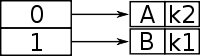
\includegraphics[width=35mm]{ExtendibleHashing.png}\\*
Laat de hashwaarde van $k1 = 010110$ en de hashwaarde van $k2 = 010110$. Deze twee hashwaarden zijn gesorteerd volgens hun eerste bit. Beide buckets worden dus ge\"identificeerd volgens hun eerste bit. Hun lokale index $d'$ is 1.\\*
Wanneer $k3 = 110110$ moet worden toegevoegd, zal er overloop zijn in de tweede bucket. Vandaar dat deze bucket moet opgesplitst worden:\\*
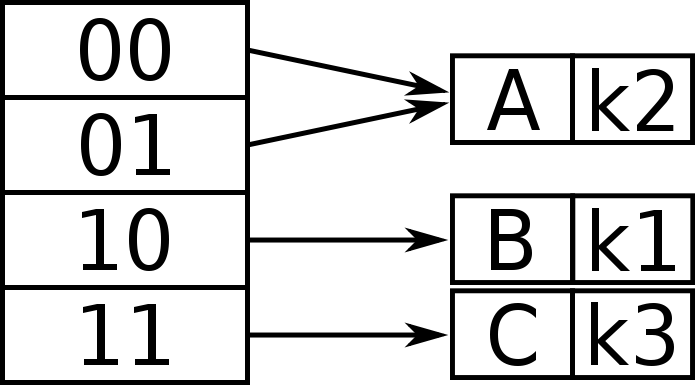
\includegraphics[width=35mm]{ExtendibleHashing2.png}\\*
De index van de eerste bucket blijft 1, deze van de tweede en derde bucket worden 2. De globale index $d$ (de index van de hashtabel), is steeds de grootste lokale index. Logischerwijs bevat de hashtabel $2^d$ elementen.\\\\
\textcolor{green}{hashtabel blijft klein}\\*
\textcolor{green}{uitbreiden van bestand is goedkoop (cel in twee splitsen)}\\*
\textcolor{red}{verdubbeling van tabel vraagt veel werk}\\*
\textcolor{red}{1 extra indirectie (te verwaarlozen)}
\section{Lineaire hashing}
Lineaire hasing begint met $M$ cellen (traditioneel een macht van 2).\\*
De eerste hashfunctie die gebruikt wordt is $h_0 = k\mod{M}$. Het aantal cellen kan varieren. Dat wil dus zeggen dat de hashfunctie ook varieert.\\*
In geval van overloop, gebruik ketening.\\*
Begin met index $i = 0$ en variabele $n = 0$.\\*
Indien een bepaalde load factor wordt overschreden (het aantal gebruikte cellen/het totaal aantal cellen), voeg een cel toe. Maak een nieuwe hashwaarde $h_{i+1} = k\mod{2^{i+1}M}$ en hoog $n$ op. Alle elementen die voor de cel $n$ zitten, daarvan zullen de hashwaarden opnieuw moeten berekend worden via de nieuwe hashfunctie $i+1$. Indien $n$ groter wordt dan $2^i*M$, hoog dan $i$ op. Zet $n = 0$. Bereken $h_0$ en $h_1$ opnieuw.\\\\
Voorbeeld:\\*
Aantal elementen per bucket = 2\\*
Split als load factor $>$ 0.7\\*
Initialiseer M = 4\\*
Toe te voegen: 5, 9, 3, 6, 22, 4, 7\\*\\*
\textit{Initialiseer, M = 4, i = 0, n = 0, load factor = 0 $<$ 0.7}\\*
\begin{tabular}{| c | c | c | c |} \hline
   &  &  &\\ \hline
   &  &  &\\ \hline
\end{tabular}\\\\
\textit{Voeg toe: 5, M = 4, i = 0, n = 0, load factor = 1/8 $<$ 0.7}\\*
\textit{Eerste hashfunctie: $h_0 = k\mod{4}, h_0(5) = 1$}\\*
\begin{tabular}{| c | c | c | c |} \hline
   & 5 &  &\\ \hline
   &  &  &\\ \hline
\end{tabular}\\\\
\textit{Voeg toe: 9, M = 4, i = 0, n = 0, load factor = 1/4 $<$ 0.7}\\*
\textit{$h_0(9) = 1$}\\*
\begin{tabular}{| c | c | c | c |} \hline
   & 5 &  &\\ \hline
   & 9 &  &\\ \hline
\end{tabular}\\\\
\textit{Voeg toe: 3, M = 4, i = 0, n = 0, load factor = 3/8 $<$ 0.7}\\*
\textit{$h_0(3) = 3$}\\*
\begin{tabular}{| c | c | c | c |} \hline
   & 5 &  & 3\\ \hline
   & 9 &  &\\ \hline
\end{tabular}\\\\
\textit{Voeg toe: 6, M = 4, i = 0, n = 0, load factor = 1/2 $<$ 0.7}\\*
\textit{$h_0(6) = 2$}\\*
\begin{tabular}{| c | c | c | c |} \hline
   & 5 & 6 & 3\\ \hline
   & 9 &  &\\ \hline
\end{tabular}\\\\
\textit{Voeg toe: 22, M = 4, i = 0, n = 0, load factor = 5/8 $<$ 0.7}\\*
\textit{$h_0(22) = 2$}\\*
\begin{tabular}{| c | c | c | c |} \hline
   & 5 & 6 & 3\\ \hline
   & 9 & 22 &\\ \hline
\end{tabular}\\\\
\textit{Voeg toe: 4, M = 4, i = 0, n = 0, load factor = 3/4 $>$ 0.7 $\rightarrow$ split!}\\*
\textit{$h_0(4) = 0$}\\*
\begin{tabular}{| c | c | c | c |} \hline
  4 & 5 & 6 & 3\\ \hline
   & 9 & 22 &\\ \hline
\end{tabular} $\rightarrow$
\begin{tabular}{| c | c | c | c | c |} \hline
   & 5 & 6 & 3 & 4\\ \hline
   & 9 & 22 & & \\ \hline
\end{tabular}\\*
\textit{M = 4, i = 0, n = 1, load factor = 3/5 $<$ 0.7}\\*
\textit{$h_1 = k\mod{2M}$}\\*
\textit{$h_1(4) = 4$}\\\\
\textit{Voeg toe: 7, M = 4, i = 0, n = 1, load factor = 7/10 $=$ 0.7}\\*
\textit{$h_0(7) = 3$}\\*
\begin{tabular}{| c | c | c | c | c |} \hline
   & 5 & 6 & 3 & 4\\ \hline
   & 9 & 22 & 7 & \\ \hline
\end{tabular}
\section{Indexstructuren}
\textbf{Index}: Een gegevensstructuur die de toegang op dat bestand via een bepaald veld effici\"enter maakt.\\*
Deze index kan opgeslagen zijn in een centraal gegeugen of in een bestand in een extern geheugen.
\subsection{Soorten indexen}
\textbf{Primaire index}: Index op het veld dat de ordening van het bestand bepaalt.\\*
De records zijn uniek.\\
\textbf{Clusterindex}: Index op het veld dat de ordening van het bestand bepaalt.\\*
De records zijn niet noodzakelijk uniek.\\
\textbf{Secundaire index}: Index op een ander veld dan het veld dat de ordening van het bestand bepaalt.
\subsubsection{Primaire indexen}
\begin{itemize}
\item Geordend volgens sleutelwaarden
\item Index bevat 1 record per blok: "ankerrecord" (= eerste of laatste record in een blok) en het adres
\end{itemize}
\textcolor{red}{Blok heeft vaste lengte $\rightarrow$ overloop}\\*
\textcolor{red}{Ankerrecords kunnen veranderen!}\\*
Oplossing: overloopgebieden en markering\\\\
Performantie:\\*
$\#$ records = $r$\\*
$\#$ blokken = $b$\\*
recordlengte = $R$\\*
bloklengte = $B$\\*
blocking factor $bfr = \lfloor B/R \rfloor$\\*
De performantie wordt weergegeven door het aantal schijftoegangen bij binair zoeken. = $\lceil \log_2{b} \rceil = \lceil \log_2{\lfloor r/bfr \rfloor} \rceil$.
\subsubsection{Clusterindex}
Geordend volgens niet-uniek veld.\\*
Aangezien er meerdere velden dezelfde waarden hebben, wijst de clusterindex naar de eerste blok dat deze waarde bevat.\\
\textcolor{red}{Bij toevoeging zouden de indexen kunnen veranderen.}\\*
Oplossing: Voor elke waarde een aparte blok gebruiken.
\subsubsection{Secundaire index}
\textbf{Sleutelveld}\\*
De index verwijst naar een sleutelveld dat niet geordend is. Maar de index zelf is wel geordend.\\*
De index kan heel groot worden, maar aangezien deze geordend is, is binair zoeken mogelijk.\\*
De performantie wordt op dezelfde manier berekend als bij de primaire index.\\\\
\textbf{Niet-sleutelveld}\\*
De index verwijst onrechtstreeks naar een niet-sleutelveld dat niet geordend is. De index zelfd is wel geordend.\\*
De index verwijst naar een blok recordwijzers.\\*
Deze blok recordwijzers verwijzen naar dezelfde sleutels in het bestand (niet-sleutelvelden zijn niet meer uniek). Dit zorgt voor 1 indirectie meer.
\subsection{Meerdere niveau's}
Principe: Index bouwen bovenop index.\\*
De blocking factor $bfr_i$ is even groot voor alle indexen (= "fan-out" $fo$).\\*
Aantal blokken op niveau $k$ = $\lceil r_1/fo^k \rceil$ ($r_1$ = aantal records op niveau 1 = totaal aantal records)\\
\textcolor{green}{snelle toegang tot bestand, toevoeging en weglating effici\"ent}\\*
\textcolor{red}{overloop is vertragend en verkwist ruimte + verplichte reorganisatie vraagt tijd}
\subsection{Boomstructuren}
Gewone binaire zoekboom is effici\"ent, maar is ongebalanceerd.
\subsubsection{B-bomen}
B-boom van orde $p$, is een zoekboom waarvoor geldt dat:\\*
\begin{itemize}
\item de wortel heeft minstens 2 knopen;
\item elke andere knoop heeft minstens $\lceil p/2 \rceil$ en maximum $p$ kinderen;
\item alle bladeren zitten even diep.
\end{itemize}
Maximale hoogte $h = \log_{\lceil p/2 \rceil}{(n+1)/2}$\\\\
Berekening van de orde van een B-boom:\\*
orde = $p$\\*
grootte blokadres = $P$\\*
grootte veld = $V$\\*
grootte recordadres = $R$\\*
grootte blok = $B$\\*
Elke knoop moet binnen 1 blok passen. Dat wil zeggen: orde*blokadres + (orde-1)*(veld+record) = blokgrootte\\*
Of: $pP+(p-1)(V+R) = B$\\\\
Typisch voor een B-boom is dat de $fo$ klein is. Hierdoor is deze boom enkel bruikbaar wanneer er met een klein aantal records, of een kleine recordgrootte wordt gewerkt.
\subsubsection{B$^+$-bomen}
Recordadressen enkel in knopen, niet meer in interne knopen. Dit zorgt ervoor dat de orde van de interne knopen veel groter is.\\*
Aan het einde van elk blad: een wijzer naar het volgende blad (voor sequenti\"ele doorloop).\\*
Orde van de interne knopen:\\*
$pP+(p-1)V = B$\\*
Orde van de bladeren:\\*
$p(V+R)+P = B$\\\\
Toevoegen van een sleutel:\\*
Indien blad vol: Splits blad in de helft. De eerste helft (afgerond naar boven) blijft, de tweede helft wordt een nieuw blad. De laatste waarde van de eerste helft moet toegevoegd worden aan ouderknoop. (Indien ouderknoop vol, doe recursief hetzelfde).\\
Verwijderen van een sleutel:\\*
Indien de sleutel ergens in de interne knopen voorkomt: vervang door de waarde net links ervan.\\*
Indien er onderloop optreedt: steel enkele waarden van een naburig blad, voeg eventueel 2 bladeren samen en verwijder 1 wegwijzer uit bovenliggende knoop.\\*
Indien onderloop in interne knoop: herverdeel
\subsubsection{B$^*$-bomen}
Elke knoop is minstens 2/3 gevuld.\\*
Splits wanneer 2 naburige knopen vol zijn.
\subsection{Indexen op meerdere velden}
Velden combineren door meerdere velden als 1 veld te beschouwen of door "partitioned hashing" (= resultaat is combinatie van aparte hashfuncties).\\*
In plaats van rijen met adressen, nu matrices met adressen.
\section{Begrippen van transactieverwerking}
\textbf{Transactie}: De uitvoering van een programma dat een gegevensbank raadpleegt of wijzigt.\\*
\textbf{Interleaved uitvoering}: serieel\\*
\textbf{Simultane uitvoering}: parallel\\*
We zullen ons verder baseren op interleaved uitvoering.\\*
\textbf{Concurrentie}: De gelijktijdige uitvoering van transacties.\\*
In geval van concurrentie kunnen er aanpassingen verloren gaan waardoor bepaalde gegevens niet meer correct zijn.\\*
\textbf{Dirty read}: Een transactie schrijft iets weg en faalt. De gewijzigde waarden worden opnieuw hersteld, maar ondertussen heeft een andere transactie deze foute waarden al gebruikt.\\*
\textbf{Foutieve sommering}: Sommige waarden van voor en sommige van na een wijziging worden opgeteld.\\*
\textbf{Niet herhaalbare lezing}: Twee maal dezelfde waarde lezen levert een ander resultaat op.
\subsection{Herstel}
\textbf{Herstel}: Een transactie moet ofwel volledig uitgevoerd worden ofwel helemaal niet.\\*
\textbf{Systeemlog}: Noteert alle transacties die waarden in een gegevensbank wijzigen.\\\\
Herstellen na faling:
\begin{itemize}
\item Transactie volledig ongedaan maken (UNDO).
\item Transactie goed afwerken (REDO).
\end{itemize}
Wat te kiezen? Commit point: Punt waarop beslist wordt dat de transactie goed afgewerkt moet worden in plaats van ongedaan gemaakt.\\*
Commit point wordt bereikt indien alle bewerkingen van de transactie met succes zijn uitgevoerd en alle bewerkingen ook op de log zijn geregistreerd.\\\\
Transacties moeten 'ACID' zijn.\\*
Atomicity (ondeelbaarheid)\\*
Consistency preservation (databank moet consistent blijven)\\*
Isolation (geen interferentie met andere transacties)\\*
Durability (effect mag niet verloren gaan)
\subsection{Transactieroosters}
2 operaties \textbf{conflicteren} indien er ten minste \'e\'en write wordt uitgevoerd door 2 verschillende transacties op hetzelfde gegevenselement.\\
Een rooster $S$ voor $n$ transacties $T_i$ is \textbf{volledig} als dit rooster alle operaties van de transacties $T_i$ bevat, de volgorde van de operaties binnen $T_i$ behoudt en de volgorde vastligt voor elk paar conflicterende operaties.\\*
Een rooster is \textbf{herstelbaar} $\Leftrightarrow$ een transactie die gecommit is, nooit meer ongedaan moet worden gemaakt.\\*
\textbf{Cascading rollback}: Een transactie terugrollen kan ervoor zorgen dat er nog meer transacties moeten teruggerolled worden.\\*
\textbf{Cascadeloze roosters}: Garanderen dat er geen cascading rollbacks nodig zijn.\\*
Voldoende voorwaarde: Elke transactie leest enkel waarden geschreven door transacties die al gecommit hebben.\\*
\textbf{Strikte roosters}: Elke transactie leest en schrijft enkel waarden die geschreven zijn door transacties die al gecommit hebben.
\subsection{Serialiseren van roosters}
\textbf{Serieel rooster}: De transacties worden na elkaar uitgevoerd.\\*
\textcolor{red}{Beperking op concurrentie.}\\
Een rooster is \textbf{serialiseerbaar} indien het rooster equivalent is met een serieel rooster (dat dezelfde transacties bevat).\\*
Verschillende soorten equivalentie:
\begin{itemize}
\item resultaat-equivalent: gegeven beginvoorwaarden, zelfde resultaat (te zwak, twee verschillende functies kunnen toevallig hetzelfde resultaat geven)
\item conflict-equivalent (conflict-serialiseerbaar): volgorde van twee conflicterende operaties steeds hetzelfde in beide roosters.
\item view-equivalent (view-serialiseerbaar): Elke overeenkomstige leesopdracht in $S_1$ leest dezelfde waarden als in $S_2$ en de laatst geschreven waarde voor een item is in beide roosters hetzelfde.
\end{itemize}
Conflict-serialiseerbaarheid is te testen met "\textbf{precedence-graph"}. Dit is een graaf die de volgorde van de transacties aanduidt.\\*
Precedence-graph:
\begin{itemize}
\item Maak voor elke transactie een knoop.
\item Maak een boog van $T_i$ naar $T_j$. Als $T_j$ een $read(X)$ na een $write(X)$, een $write(X)$ na een $read(X)$ of een $write(X)$ na een $write(X)$ van $T_i$ uitvoert.
\item Het rooster is serialiseerbaar $\Leftrightarrow$ er zijn geen cycli.
\end{itemize}
Problemen met testen van serialiseerbaarheid:
\begin{itemize}
\item Interleaving van operaties wordt bepaald door het besturingssysteem.
\item Transacties worden continu aangeboden: Het begin en einde van de roosters is moeilijk te voorspellen.
\end{itemize}
Het is dus beter om bij het opstellen van de transacties serialiseerbaarheid te garanderen.
\section{Transactiecontrole II: Technieken voor concurrentiecontrole en herstel}
\subsection{Concurrentiecontrole - Locking}
Een \textbf{grendel (lock)} is een variable dat bij de gegevensbank hoort en de status beschrijft van een element.
\subsubsection{Binaire grendels}
2 toestanden:\\*
$lock(X) = 1$: X is niet toegankelijk\\*
$lock(X) = 0$: X is wel toegankelijk\\*
2 bewerkingen:\\*
$lock\_item(X)$: een transactie vraagt toegang tot $X$\\*
$unlock\_item(X)$: een transactie geeft $X$ weer vrij\\\\
Regels voor vergrendeling:\\*
$T$ moet:
\begin{itemize}
\item $lock\_item(X)$ uitvoeren voor $read\_item(X)$ of $write\_item(X)$
\item $unlock\_item(X)$ uitvoeren nadat alle $read\_item(X)$ of $write\_item(X)$ uitgevoerd zijn
\end{itemize}
$T$ mag geen:
\begin{itemize}
\item $lock\_item(X)$ uitvoeren als het al een grendel heeft op $X$
\item $unlock\_item(X)$ uitvoeren als het geen grendel heeft op $X$
\end{itemize}
\subsubsection{Read/write locks}
Ook gedeelde/exclusieve grendels genoemd.\\*
3 toestanden: niet vergrendeld, lees-grendel, schrijf-grendel\\*
3 bewerkingen:\\*
$read\_lock(X)$, $write\_lock(X)$ en $unlock\_item(X)$\\\\
Regels voor vergrendeling:\\*
$T$ moet:
\begin{itemize}
\item $read\_lock(X)$ of $write\_lock(X)$ uitvoeren voor een $read\_item(X)$
\item $write\_lock(X)$ uitvoeren voor een $write\_item(X)$
\item $unlock(X)$ uitvoeren nadat alle $read\_item(X)$ of $write\_item(X)$ uitgevoerd zijn
\end{itemize}
$T$ mag geen:
\begin{itemize}
\item $read\_lock(X)$ of $write\_lock(X)$ uitvoeren als het al een grendel heeft op $X$
\item $unlock\_item(X)$ uitvoeren als het geen grendel heeft op $X$
\end{itemize}
Conversie van grendels:\\*
Als $T$ als enige een leesgrendel heeft op $X$, dan mag deze geupgraded worden naar een schrijfgrendel.\\*
Een schrijfgrendel mag altijd gedowngraded worden naar een leesgrendel.\\\\
Lees-/schrijf-vergrendeling vermijdt bepaalde problemen, maar levert geen serialiseerbaarheid. Daarom moet er een protocol ingevoerd worden.
\subsubsection{Twee-fasen-vergrendeling}
Alle vergrendelingen van een transactie gebeuren voor de eerste ontgrendeling.\\*
\textcolor{green}{Garandeert serialiseerbaarheid.}\\*
\textcolor{red}{Vermijdt geen deadlock/starvation.}\\\\
Varianten:
\begin{itemize}
\item Basisversie: zoals hierboven gezien
\item Conservatieve versie: Alle grendels plaatsen voor de transactie begin (vermijdt deadlocks, maar grendels niet altijd op voorhand gekend).
\item Strikte/rigoureuze versie: Geen enkele grendel vrijgeven voor commit of abort (garandeert strikt rooster, maar is niet deadlockvrij).
\end{itemize}
\subsection{Concurrentiecontrole - Timestamps}
Deadlock prevention: Conservatieve 2FV (grote beperking op concurrentie) of het gebruik van tijdstempels.\\
Tijdstempels: $T_1$ start voor $T_2$: $TS(T_1) < TS(T_2)$\\
Mogelijke schema's:
\begin{itemize}
\item wait-die schema: als $TS(T_i) < TS(T_j)$, dan moet $T_i$ wachten tot er een grendel vrijkomt, anders wordt $T_j$ afgebroken en later terug herstart met dezelfde tijdstempel.
\item wound-wait schema: als $TS(T_i) < TS(T_j)$, dan wordt $T_j$ afgebroken, anders moet deze wachten tot er een grendel bijkomt.
\end{itemize}
\begin{center}
\begin{tabular}{| c | c | c |} \hline
  & Wait/Die & Wound/Wait \\\hline
 $Y_i$ needs a resource held by $Y_j$ & $Y_i$ waits & $Y_j$ dies \\\hline
 $Y_j$ needs a resource held by $Y_i$ & $Y_j$ dies & $Y_j$ waits \\\hline
\end{tabular}
\end{center}
\textcolor{green}{De jongste transactie is degene die altijd afgebroken wordt $\rightarrow$ minder werk gaat verloren.}\\*
\textcolor{green}{Deadlock -en starvation-vrij}\\*
\textcolor{red}{Sommige transacties worden onnodig afgebroken.}
\subsubsection{Deadlock preventie zonder timestamps}
\begin{itemize}
\item "No waiting" schema: Transactie onmiddelijk afbreken indien deze een grendel niet kan krijgen.
\item "Cautious waiting" schema:  Transactie mag enkel wachten op een grendel indien de transactie die deze grendel heeft zelf niet aan het wachten is. (Is deadlockvrij)
\item Timeouts: Transactie te lang aan het wachten: afbreken en herstarten.
\end{itemize}
\subsubsection{Deadlock detectie}
Detectie op basis van de "wacht op" graaf. Lus in graaf = deadlock.\\*
Indien deadlock: Kies een slachtoffer om af te breken. Maar: Starvation.\\*
Oplossingen voor starvation:
\begin{itemize}
\item Eerlijke toekenning van grendels (first come, first serve; verschillende prioriteiten)
\item Eerlijke slachtofferselectie.
\end{itemize}
\subsubsection{Concurrentiecontrole zonder grendels}
Serialiseerbaarheid garanderen d.m.v. tijdstempels.\\\\
Twee tijdstempels:\\*
$read\_TS(X)$: Tijdstempel van de jongste transactie die $X$ heeft gelezen.\\*
$write\_TS(X)$: Hetzelfde voor schrijven.\\
Voorbeeld: $T$ mag $X$ niet lezen of schrijven als $X$ door een transactie met latere tijdstempel geschreven is.\\\\
Indien tijdstempels niet kloppen: Transactie ongedaan maken en opnieuw aanbieden (met latere tijdstempel) $\rightarrow$ Cascading rollback.\\\\
Vermijdt deadlock, maar geen starvation. Het tijdstempelordeningsalgoritme is bovendien niet herstelbaar.\\\\
Strikte tijdstempelordening:\\*
Er wordt gewacht met $read(X)$ of $write(X)$ totdat de transactie met timestamp $write\_item(X)$ gecommit of afgebroken is.
\subsection{Concurrentiecontrole - Multiversietechnieken}
Als $T$ een $write(X)$ mag uitvoeren: creatie van een nieuwe versie $X_{k+1}$ met $read\_TS(X_{k+1})$, $write\_TS(X_{k+1})$ = $TS(T)$\\*
Als $T$ de waarde van versie $X_i$ mag lezen:\\*
$read\_TS(X_i)$ = $max(read\_TS(X_i), TS(T))$
\subsection{Concurrentiecontrole - Optimistische concurrentiecontrole}
Alle aanpassingen gebeuren in lokale kopies.\\*
Valideringsfase: Indien aan serialiseerbaarheid voldaan: commit, anders herstart later opnieuw.
\subsection{Concurrentiecontrole - Granulariteit van gegevensitems}
Granulariteit = grootte van de gegevens\\*
Databank = grove granulariteit, veld in een record = fijne granulariteit\\*
Hoe fijner de granulariteit, hoe meer concurrentie mogelijk is.
\subsection{Herstel - Begrippen}
\textbf{Immediate update}: Wijzigingen kunnen aangebracht worden voor het bereiken van een commit point.\\*
\textbf{Deferred update}: Wijzigingen pas aanbrengen na het bereiken van een commit point.\\
DBMS systemen gebruiken cache als buffer.\\*
\textbf{Dirty bit}: Geeft aan of een pagina gewijzigd is.\\*
\textbf{Pin/unpin bit}: Geeft aan of pagina teruggeschreven mag worden naar disk (pin zolang een transactie nog werk heeft).\\\\
\textbf{Write-ahead logging}: Eerst naar log schrijven, dan pas aanpassing doorvoeren.\\*
\textbf{Steal}: Pagina naar schijf schrijven, ook al is deze vastgepind.\\*
\textbf{Force}: Alle gewijzigde pagina's onmiddelijk naar schijf schrijven.\\\\
\textbf{Checkpoint}: Alle gewijzigde buffers worden naar schijf geschreven. Checkpoint wordt op de log geschreven.\\*
\textbf{Fuzzy checkpoint}: Wanneer alles geschreven is op de log, transacties hervatten (vorige checkpoint blijft nog even bestaan).
\subsection{Herstel - Hersteltechnieken [uitgestelde aanpassing]}
Een transactie kan de gegevensbank niet wijzigen voor het bereiken van haar commit point.\\*
Een transactie bereikt haar commit point vooraleer aanpassingsopdrachten zijn geregistreerd op de log.\\*
NO-UNDO/REDO algoritme. (RDU\_M)\\*
Effici\"entere versie:\\*
Enkel de laatste write van een item doorvoeren. De log achterstevoren doorlopen en REDO $write(X)$ enkel indien eerder (verder op de log) nog geen $write(X)$ tegengekomen is.
\subsection{Herstel - Hersteltechnieken [onmiddelijke aanpassing]}
Wijzigingen gebeuren in de database zelf.\\*
Write-ahead log protocol.\\*
REDO/UNDO. (RIU\_S)
\subsection{Herstel - Schaduwpaginering}
Construeer een index voor de relevante delen van de database. Kopi\"eer deze painatabel naar de schijf (= schaduwindex).\\*
Gedurende de transactie wordt de paginatabel aangepast, maar de originele schaduwindex blijft ongewijzigd.\\*
Bij een commit verdwijnt deze schaduwindex.
\end{document}